%\documentclass[11pt,a4paper]{article}
\documentclass[11pt
  , a4paper
  , article
  , oneside
%  , twoside
%  , draft
]{memoir}

\usepackage{control}
\usepackage[numbers]{natbib}

\newcommand{\newappendix}{%
  \refstepcounter{chapter}\chapter*{Appendix \thechapter}%
  \addcontentsline{toc}{chapter}{Appendix \thechapter}%
}

\begin{document}

\newcommand{\technumber}{
  RAON Control-Document Series\\
  Revision : v1.0,   Release : June 24, 2014}
\title{\textbf{Classic Channel Archiver 설정 메뉴얼}}

\author{손 창욱\thanks{scwook@ibs.re.kr} \\

  Rare Isotope Science Project\\
  Institute for Basic Science, Daejeon, South Korea
}
\date{\today}

\renewcommand{\maketitlehooka}{\begin{flushright}\textsf{\technumber}\end{flushright}}
%\renewcommand{\maketitlehookb}{\centering\textsf{\subtitle}}
%\renewcommand{\maketitlehookc}{C}
%\renewcommand{\maketitlehookd}{D}

\maketitle

\begin{abstract}
Classic Channel Archiver는 EPICS의 ChannelAccess를 통해 각 device에 대한 Channel정보를
일련의 파일로 저장하는 툴이다. 본 메뉴얼은 Classic Channel Archiver의 Main Engine인 ArchiveEngine 및 
Engine Configuration, 저장된 Data를 Retrieval하기 위한 DataServer Configuration을 포함하고 있으며
Channel Archiver Manual\citep{CA_MANUAL}을 바탕으로 작성되었다.
\end{abstract}

\chapter{Sample Mechanisms}
\section{Monitored Sampling}
Monitor Mode의 경우 Archive Engine(AE)은 Channel Access(CA) 서버에게 monitor요청을 하게 된다.
즉, CA 서버는 채널 값이 변경되면 AE에게 알리게 되고 이 때 채널 값을 저장하게 된다. 결과적으로
Monitor Mode는 채널 값이 변경될때 마다 저장하는 방식이다. 이 모드의 경우 다음 몇 가지 문제점이
있다.
\begin{itemize}
\item 채널 값이 변하지 않는 경우 Archive가 되지 않는다. 
\item 채널 값이 빠르게 변할 경우 데이터 용량이 커진다.
\end{itemize} 
\section{Scanned Sampling}
Scan Mode의 AE는 채널 값을 CA 서버에게 주기적으로 요청한다. 이 경우 Monitor Mode와 달리
채널 값이 변하지 않더라도 값을 저장하게 된다. 하지만 동일한 값이 계속 저장되면 저장공간 낭비가
발생 하므로 AE는 이전 값과 같은 값이 반복되어 들어오면 'repeat count'를 저장하여 공간을 절약한다.
Scan Mode의 경우 다음과 같은 문제점이 있다.
\begin{itemize}
\item 'fault' 정보를 가지고 있는 채널에 대해서는 적합하지 않다. 만약 'fault'가 scan 주기 사이에
발생하게 되면 AE는 이 값을 저장할 수 없다.
\item AE는 CA 서버에게 주기적으로 요청하므로 네트워크 부하가 발생할 수 있다. 따라서 Scan Mode는
1분 또는 그 이상의 주기를 가지는 Archive에 대해 적합하다.
\item 네트워크 지연 및 record의 주기등과 같은 이유로 채널의 시간에 오차가 발생할 수 있다.
\end{itemize} 
\section{Scanned using Monitors}
Scan과 Monitor Mode를 합쳐놓은 것으로 AE의 설정에 따라 Scan 또는 Monitor Mode로 작동한다.
예를 들어 IOC의 record값이 1초 주기로 변경되는 경우에 대해 30초 마다 저장하고자 하면
Scan Mode가 효율적이다. 하지만 만약 5초 마다 저장할 경우 네트워크 부하를 줄이기 위해
Monitor Mode가 더 적합하다. 즉 CA 서버로 부터 1초마다 채널 정보를 받아 1개의 값만 저장하고
4개의 값을 무시하는 방법이 효율적이다.
이 방법은 Scan Mode에서 작동하며 AE의 설정 값중 get\_threshold 값에 따라 결정 된다.
만약 Scan 주기가 get\_threshold 보다 작을 경우 Channel 값은 Monitor Mode로 전환되어 작동한다.
이 방법은 다음과 같은 문제점이 있다.
\begin{itemize}
\item 1 또는 30초 주기를 가지는 Scan의 경우 일반적인 Scan Mode보다 네트워크 부하가 작은 장점이
있지만 여전히 'repeat count'에 대한 정보를 위해 CA 서버에 채널값에 대한 요청이 필요하다. 만약
0.1초 주기와 같이 빠른 경우 일반적인 Monitor Mode에 비해 CPU 부하가 커질 수 있다.
\end{itemize}
\chapter{설치}
Channel Archiver를 설치하기 위해서는 기본적으로 EPICS Base 및 Extenstion이 설치 되어 있어야 한다.
본 메뉴얼에서는 다음 EPICS 구조를 따라 설치를 진행하였다.
\begin{itemize}
  \item \texttt{EPICS Structure}
    {\scriptsize
     \begin{verbatim}
      ctrluser@ctrluser $
      epics
      ├── downloads
      └── R3.14.12.4
          ├── base
          ├── epicsLibs
          ├── extensions
          ├── siteApps
          └── siteLibs
     \end{verbatim}
     }
\end{itemize}
Channel Archiver의 기본 설치는 홈페이지\citep{CA_HOME}또는 Web Repositories\citep{CA_SF}에서
소스코드를 다운 받은 후 컴파일 하면된다. 현재 CA는 2006년 이후 새로운 버전이 개발되지
않고 있어 Update된 Library 및 Compiler환경에 따른 Compile 오류가 많이 발생한다. 
따라서 현재 개발 환경에 맞는 코드 수정이 필요하며 다음 Script를 이용하면 쉽게 설치가 가능한다.\\
Script실행에 앞서 필요한 Library를 설치한다.
\begin{lstlisting}[style=termstyle]
ctrluser@ctrluser:~$ aptitude install libxmlrpc-c++4-dev libxerces-c2-dev libcurl3-dev
\end{lstlisting}
script를 실행하여 설치를 진행한다.
\begin{lstlisting}[style=termstyle]
ctrluser@ctrluser:~$ bash chanarch.sh
\end{lstlisting}
설치가 완료되면 extension/src/ChannelArchiver에 소스코드가 설치되고 extension/bin/linux-x86\_64 안에 
Archive Engine를 포함한 실행파일들이 위치하게 된다.
\chapter{Archive Engine}
\section{Configuration}
Archive Engine을 시작하기 전 저장하고자 하는 Channel리스트, 주기, 데이터 파일 크기와 같은
기본 설정이 필요하며 이러한 설정들은 XML-type의 파일에 정의된다. XML파일을 만들기 앞서
파일 구조를 설정하는 engineconfig.dtd파일을 만든다.
\begin{lstlisting}[style=termstyle]
<?xml version="1.0" encoding="UTF-8"?>
<!-- DTD for the ArchiveEngine Configuration         -->
<!-- Note that we do not allow empty configurations: -->
<!-- Each config. must contain at least one group,   -->
<!-- and each group must contain at least 1 channel. -->
<!ELEMENT engineconfig ((write_period|get_threshold|
                         file_size|ignored_future|
                         buffer_reserve|
                         max_repeat_count|disconnect)*,
                         group+)>
<!ELEMENT group (name,channel+)>
<!ELEMENT channel (name,period,(scan|monitor),disable?)>
<!ELEMENT write_period (#PCDATA)><!-- int seconds -->
<!ELEMENT get_threshold (#PCDATA)><!-- int seconds -->
<!ELEMENT file_size (#PCDATA)><!-- MB -->
<!ELEMENT ignored_future (#PCDATA)><!-- double hours -->
<!ELEMENT buffer_reserve (#PCDATA)><!-- int times -->
<!ELEMENT max_repeat_count (#PCDATA)><!-- int times -->
<!ELEMENT disconnect EMPTY>
<!ELEMENT name (#PCDATA)>
<!ELEMENT period (#PCDATA)><!-- double seconds -->
<!ELEMENT scan EMPTY>
<!ELEMENT monitor EMPTY>
<!ELEMENT disable EMPTY>
\end{lstlisting} 
이제 앞서만든 DTD파일 구조를 따르는 engineconfig.xml파일을 생성한 후 값을 설정한다.
\begin{lstlisting}[style=termstyle]
<?xml version="1.0" encoding="UTF-8" standalone="no"?>
<!DOCTYPE engineconfig SYSTEM "engineconfig.dtd">
<engineconfig>
   <write_period>30 sec</write_period>
   <get_threshold>10 sec</get_threshold>
   <file_size>30</file_size>
   <ignored_future>1 hour</ignored_future>
   <buffer_reserve>3</buffer_reserve>
   <max_repeat_count>120</max_repeat_count>
   <group>
      <name>AB</name>
      <channel><name>ab:TEM</name>
               <period>1 sec</period><scan/>
      </channel>
      <channel><name>ab:HUM</name>
              <period>1 sec</period><scan/>
      </channel>
   </group>
</engineconfig>
\end{lstlisting}

\subsection{write\_period}
그룹 및 채널값을 데이터 파일에 쓰는 주기를 지정한다. Archive Engine은 일정시간
Buffer에 값을 저장하는데 여기에 설정된 시간이 지나면 데이터 파일에 값을 저장한다.
예를 들어 30 sec로 설정 할 경우 30초 동안 들어오는 값들을 메모리 버퍼에 저장했다가
매 30초 마다 버퍼에 있는 값들을 파일로 저장한다.

\subsection{get\_threshold}
scan mode일 경우 monitor mode로 변경되는 기준을 get\_threshold 따라 결정한다.
변경되는 기준은 period가 get\_threshol 보다 작을경우 monitor mode로 변경된다.
예를 들어 get\_threshold가 10sec로 설정되어 있을 때 period가 5 sec인 scan mode의 
channel은 monitor mode로 작동한다. 반면 period를 30 sec로 변경 할 경우 scan mode 그대로
작동한다.
\subsection{file\_size}
데이터 파일 크기를 지정한다. 예를 들어 100으로 설정 할 경우 데이터 파일이 100MB가 되면
새로운 파일을 생성 한다.

\subsection{ignored\_future}
Channel로 부터 저장되는 시간이 ``현재 시간 + ignored\_future'' 시간 범위를 벗어나는 경우
들어오는 Channel값들을 무시한다. 

\subsection{buffer\_reserve}
메모리 버퍼 크기를 지정한다. 전체 버퍼 크기는 다음 수식에 따라 정해진다.\\
\newline
buffer reserve x write period / scan period
\newline

\subsection{max\_repeat\_count}
scanned mode의 경우 반복되는 값에 대한 count 최대 값을 지정한다. 

\subsection{disconnect}
disable 채널에 대한 연결 유지 유무를 설정한다. 기본 설정으로 disable 채널들은
조건을 만족할 때 그룹에 대한 Archive를 비활성화 시키지만 자신은 Channel Access를 통해
연결을 유지하고 있다. 만약 disconnect 설정이 되어있다면 이러한 disable 채널들에 대한
Channel Access연결 또한 해제 한다.
\subsection{group}
다수의 채널을 그룹으로 묶어 관리할 수 있으며 2개의 하위 태그를 가지고 있다.
\begin{itemize}
\item name: 그룹 이름을 지정한다.
\item channel: 다음 5개의 하위 태그를 가지고 있다.
\begin{itemize}
\item name: 채널 이름을 지정한다.
\item period: 채널 값을 저장하는 주기를 지정한다.
\item scan: period에 설정된 시간 주기로 scan mode로 작동한다.
\item monitor: monitor mode로 작동한다. peroid 보다 빠른 빈도로 값이 변하면 무시한다.
\item disable: disable 태그가 설정된 channel값이 0보다 크면 같은 그룹에 속해있는 channel들의 archive가 비활성 된다.
\end{itemize}
\end{itemize}
\section{Starting and Stopping}
ArchiveEngine을 시작하기 위해 다음과 같이 실행한다.
\begin{lstlisting}[style=termstyle]
ctrluser@ctrluser:~\$ ArchiveEngine engineconfig.xml ./index
07/23/2014 13:39:57 Starting Engine with configuration file engineconfig.xml, index ./index
07/23/2014 13:39:57 Creating ChannelAccess Context.
07/23/2014 13:39:57 Engine starts.
07/23/2014 13:39:57 Starting EngineServer
07/23/2014 13:39:57 
-------------------------------------------------
Engine Running. Stop via http://localhost:4812/stop
-------------------------------------------------
07/23/2014 13:39:57 HTTPServer thread 0x01D24680 running.
\end{lstlisting}
Engine이 시작되면 중복 실행되는 것을 방지하기 위해 lock파일(archive\_active.lck)이 자동으로 생성된다.
따라서 archive\_active.lck가 존재하는 상태에서는 Engine을 시작할 수 없게된다. Engine이 중지되면 lock
파일은 자동으로 삭제되는데, 만약 시스템 오류등으로 제대로 중지되지 않을 경우 lock파일은 삭제되지 않는다.
이 경우 강제적으로 삭제하면 다시 시작할 수 있게 된다.\\
Engine을 중지하기 위해서는 키보드의 ``CTRL-C''를 누르거나 Engine을 시작할 때 나오는 웹 주소
``http://localhost:4812/stop'' 명령을 통해 중지할 수 있다.\\
여러 Engine을 동시에 시작하고자 할 경우에는 다음 2가지 사항에 따라 진행한다.
\begin{itemize}
\item Engine하나당 하나의 lcok파일만 생성되므로 각각의 폴더를 만들어서 실행시킨다.
\item 웹 서버의 TCP포트 중복을 막기 위해 ``-p \textless port\textgreater''옵션을 이용하여 서로 다른 포트를 설정한다.
\end{itemize}
웹 서버의 TCP포트는 기본 4812포트를 사용하며 ``-p'' 옵션을 통해 다음과 같이 변경이 가능하다.
\begin{lstlisting}[style=termstyle]
ctrluser@ctrluser:~\$ ArchiveEngine -p 5001 engineconfig.xml ./index
07/23/2014 14:41:44 Starting Engine with configuration file engineconfig.xml, index index
07/23/2014 14:41:44 Creating ChannelAccess Context.
07/23/2014 14:41:44 Engine starts.
07/23/2014 14:41:44 Starting EngineServer
07/23/2014 14:41:44 
-------------------------------------------------
Engine Running. Stop via http://localhost:5001/stop
-------------------------------------------------
07/23/2014 14:41:44 HTTPServer thread 0x00F419A0 running.
\end{lstlisting} 
\chapter{Data Retrieval}
Archive Engine에 의해 파일로 저장된 데이터를 읽는 방법은 크게 2가지 방법이 있다.
\begin{itemize}
\item Archive Export\\
데이터 파일에 직접 접근하여 텍스트로 출력한다.
\item Archive Data Server\\
CSS, Java Archvie Viewer와 같은 Client Tool을 이용하여 그래프로 출력한다.
\end{itemize}
\section{Archive Export}
Archive Export는 명령어 라인 툴로서 별도의 설정이 필요없이 데이터 파일에 직접 접근하여
원하는 데이터를 텍스트로 출력해 준다. 기본 적인 사용방법은 다음과 같다.
\begin{lstlisting}[style=termstyle]
USAGE: ArchiveExport [Options] <index file> {channel}

Options:
  -verbose                                   Verbose mode
  -match <reg. exp.>                         Channel name pattern
  -list                                      List all channels
  -info                                      Time-range info on channels
  -start <time>                              Format: "mm/dd/yyyy[ hh:mm:ss[.nano-secs]]"
  -end <time>                                (exclusive)
  -text                                      Include text column for status/severity (default)
  -no_text                                   Exclude text column for status/severity
  -output <file>                             Output to file
  -plotbin <seconds>                         Bin the raw data for plotting
  -average <seconds>                         average values
  -linear <seconds>                          Interpolate values linearly
  -format <decimal|engineering|exponential>  Use specific format for numbers
  -precision <int>                           Precision of numbers
  -gnuplot                                   Generate GNUPlot command file
  -Gnuplot                                   Generate GNUPlot output for Image
  -raw_time                                  Include columns for EPICS time stamp
  -millisecs                                 Truncate time to millisecs in spreadsheet dump.

\end{lstlisting}
Archive Export는 출력 형식에 따라 다양한 설정들을 지원한다. 예를 들어 채널 값을 텍스트로 출력하려면
다음과 같이 하면 된다.
\begin{lstlisting}[style=termstyle]
ctrluser@ctrluser:~\$ ArchiveExport -l index
ab:HUM
ab:TEM
ctrluser@ctrluser:~/ ArchiveExport -output data.txt index ab:HUM
ctrluser@ctrluser:~/ cat data.txt
...
...
...
06/19/2014 15:59:20.871534536	16995	
06/19/2014 15:59:21.871677190	17347	
06/19/2014 15:59:22.871693851	17140	
06/19/2014 15:59:23.871531523	17099	
06/19/2014 15:59:24.871585182	17207	
06/19/2014 15:59:25.871533847	17247	
06/19/2014 15:59:26.871683500	17197	
06/19/2014 15:59:27.871794155	17261	
06/19/2014 15:59:28.871528834	17078	
07/23/2014 14:27:17.950156693	#N/A	Archive_Off
07/23/2014 14:42:45.201544627	#N/A	Archive_Off

\end{lstlisting}
특정 시간에 대한 값을 출력하고자 한다면 다음과 같이 하면 된다.
\begin{lstlisting}[style=termstyle]
ctrluser@ctrluser:~\$ ArchiveExport -output data.txt -s "06/19/2014 15:50:00" -e "06/19/2014 15:51:00" index ab:HUM
ctrluser@ctrluser:~\$ cat data.txt
# Time                       	ab:HUM []	
06/19/2014 15:49:59.871533064	16549	
06/19/2014 15:50:00.871712716	16785	
06/19/2014 15:50:01.871538388	16933	
06/19/2014 15:50:02.871716040	17092	
06/19/2014 15:50:03.871572710	17030	
06/19/2014 15:50:04.871546374	16833	
06/19/2014 15:50:06.871567697	16833	Repeat 1
06/19/2014 15:50:06.871567697	16649	
06/19/2014 15:50:07.871731350	16869	
06/19/2014 15:50:08.871589020	16880	
06/19/2014 15:50:09.871528686	16966	
06/19/2014 15:50:10.871585345	16904	
06/19/2014 15:50:11.871530010	16711	
06/19/2014 15:50:12.871751659	16399	
06/19/2014 15:50:13.871588331	16730	
06/19/2014 15:50:15.871706648	16730	Repeat 1
06/19/2014 15:50:15.871706648	16964	
06/19/2014 15:50:16.871692311	16559	
06/19/2014 15:50:17.871672975	16588	
06/19/2014 15:50:18.871730633	16819	
06/19/2014 15:50:19.871536307	16585	
06/19/2014 15:50:20.871588966	17045	
06/19/2014 15:50:21.871520633	16935	
06/19/2014 15:50:22.871718283	16759	
06/19/2014 15:50:23.871734944	16640	
06/19/2014 15:50:24.871524619	16690	
06/19/2014 15:50:25.871732268	16719	
06/19/2014 15:50:26.871535942	16435	
06/19/2014 15:50:27.871726593	16599	
06/19/2014 15:50:28.871696257	16861	
06/19/2014 15:50:29.871511930	16642	
06/19/2014 15:50:30.871709581	16592	
06/19/2014 15:50:31.871568251	16464	
06/19/2014 15:50:32.871740903	16680	
06/19/2014 15:50:33.871731566	16516	
06/19/2014 15:50:34.871524240	16657	
06/19/2014 15:50:35.871685893	16626	
06/19/2014 15:50:36.871538564	16761	
06/19/2014 15:50:37.871751213	16457	
06/19/2014 15:50:38.871589885	16826	
06/19/2014 15:50:39.871542550	16421	
06/19/2014 15:50:40.871708202	16697	
06/19/2014 15:50:41.871565873	16688	
06/19/2014 15:50:42.871551536	16214	
06/19/2014 15:50:43.871581196	16733	
06/19/2014 15:50:44.871559860	16547	
06/19/2014 15:50:45.871697514	16683	
06/19/2014 15:50:46.871824168	16373	
06/19/2014 15:50:47.871528848	16626	
06/19/2014 15:50:48.871720499	16716	
06/19/2014 15:50:49.871531172	16669	
06/19/2014 15:50:50.871694825	16561	
06/19/2014 15:50:51.871581494	16147	
06/19/2014 15:50:52.871530159	16378	
06/19/2014 15:50:53.871723809	16516	
06/19/2014 15:50:54.871543483	16609	
06/19/2014 15:50:55.871693136	16538	
06/19/2014 15:50:56.871539807	16430	
06/19/2014 15:50:57.871711459	16509	
06/19/2014 15:50:58.871699122	16633	
06/19/2014 15:50:59.871561792	16395	
\end{lstlisting}
\section{Archive Data Server}
Data Server를 사용하기 위해서는 몇가지 설정이 필요하다.
\subsection{설치}
ArchiveDataServer를 ArchiveDataServer.cgi로 변경한 후 /var/www/html/archive/cgi/ 로 옮긴다.
serverconfig.dtd 파일을 만든 후 아래 내용을 추가한다.
\begin{lstlisting}[style=termstyle]
<?xml version="1.0" encoding="UTF-8"?>
<!-- DTD for the XML-RPC Data Server Configuration -->
<!ELEMENT serverconfig (archive+)>
<!ELEMENT archive (key,name,path)>
<!ELEMENT key (#PCDATA)>
<!ELEMENT name (#PCDATA)>
<!ELEMENT path (#PCDATA)>
\end{lstlisting}
서버 설정을 위해 serverconfig.xml 파일을 만든 후 다음 3가지 내용을 추가한다.
\begin{itemize}
\item key: 각각의 Archive에 대하여 독립적인 키값을 설정한다.
\item name: Archive 이름을 설정한다.
\item path: index파일이 위치한 경로를 설정한다.
\end{itemize}

\subsection{설정}
관리자 권한으로 /etc/apache2/apache2.conf 파일에 아래 내용을 추가한 후 서버를 재시작 한다.
\begin{lstlisting}[style=termstyle]
ctrluser@ctrluser:~\$ sudo vi /etc/atache2/apache2.conf
AddHandler cgi-script .cgi

<Directory /var/www/html/archive>
Order Allow,Deny
Allow from All
</Directory>

<Directory /var/www/html/archive>
SetEnv "EPICS_TS_MIN_WEST" "300"
SetEnv "LD_LIBRARY_PATH" "/lib:/usr/lib:/usr/local/lib:/home/ctrluser/epics/base-3.14.12.4/lib/linux-x86_64:/home/ctrluser/epics/extensions_for_3.14.12.4/lib/linux-x86_64:/usr/lib:/usr/local/lib"
SetEnv "SERVERCONFIG" "/var/www/html/archive/cgi/serverconfig.xml"
#PerlHandler Apache::Registry
#PerlSendHeader On
Options +ExecCGI
</Directory>

ctrluser@ctrlser:~\$ /etc/init.d/apache2 restart

\end{lstlisting}
\subsection{CSS 테스트}
데이터 서버 테스트를 위해 CSS를 실행 하여 다음과 같이 설정한다.
\begin{itemize}
\item Edit-Preferences를 실행.
\item CSS Applications-Trends-Data Browser 선택.
\item Archive Data Server URLs에 다음의 Data Server 주소 추가.
 \begin{itemize}
 \item xnds://10.1.5.13/html/archive/cgi/ArchiveDataServer.cgi
 \end{itemize}
\item File-Restart CSS 실행
\item CSS-Trends-Data Browser 실행
\item Archive Search URL을 설정한 Data Server로 선택
\item Pattern에 PV Name또는 *를 입력한 후 Search 클릭
\item 검색된 PV Nmae위에 마우스 오른쪽 버튼을 눌러 Process Variable-Data Broser 선택
\item Data Browser에서 Value Axes를 조정하여 Y축 범위를 PV 값에 맞게 조절한다.
\end{itemize}

\begin{figure}[!htb]
  \centering
  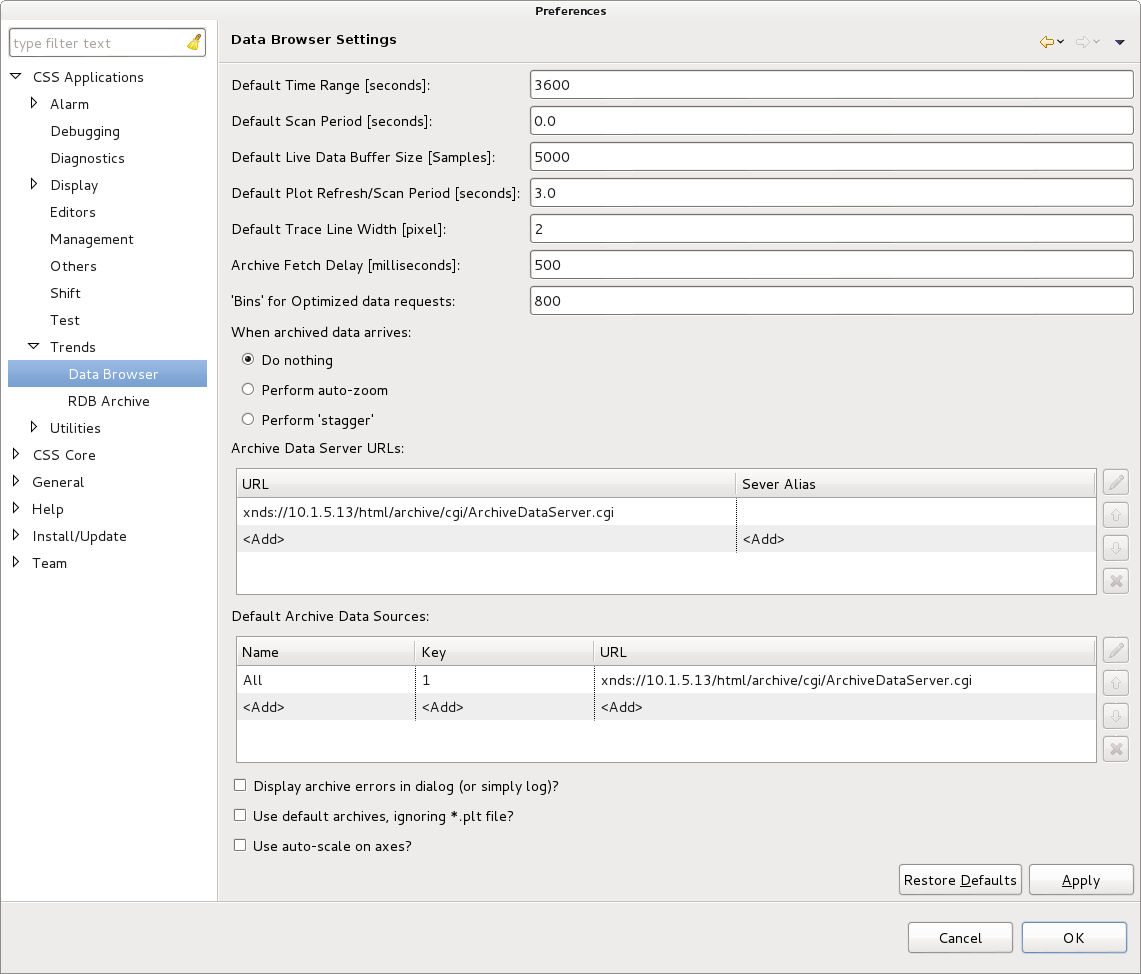
\includegraphics[width=0.96\textwidth]{./images/databrowserset.png}
  \caption{
            Data Browser Setting
          }
  \label{fig:css_db_set}
\end{figure}

\begin{figure}[!htb]
  \centering
  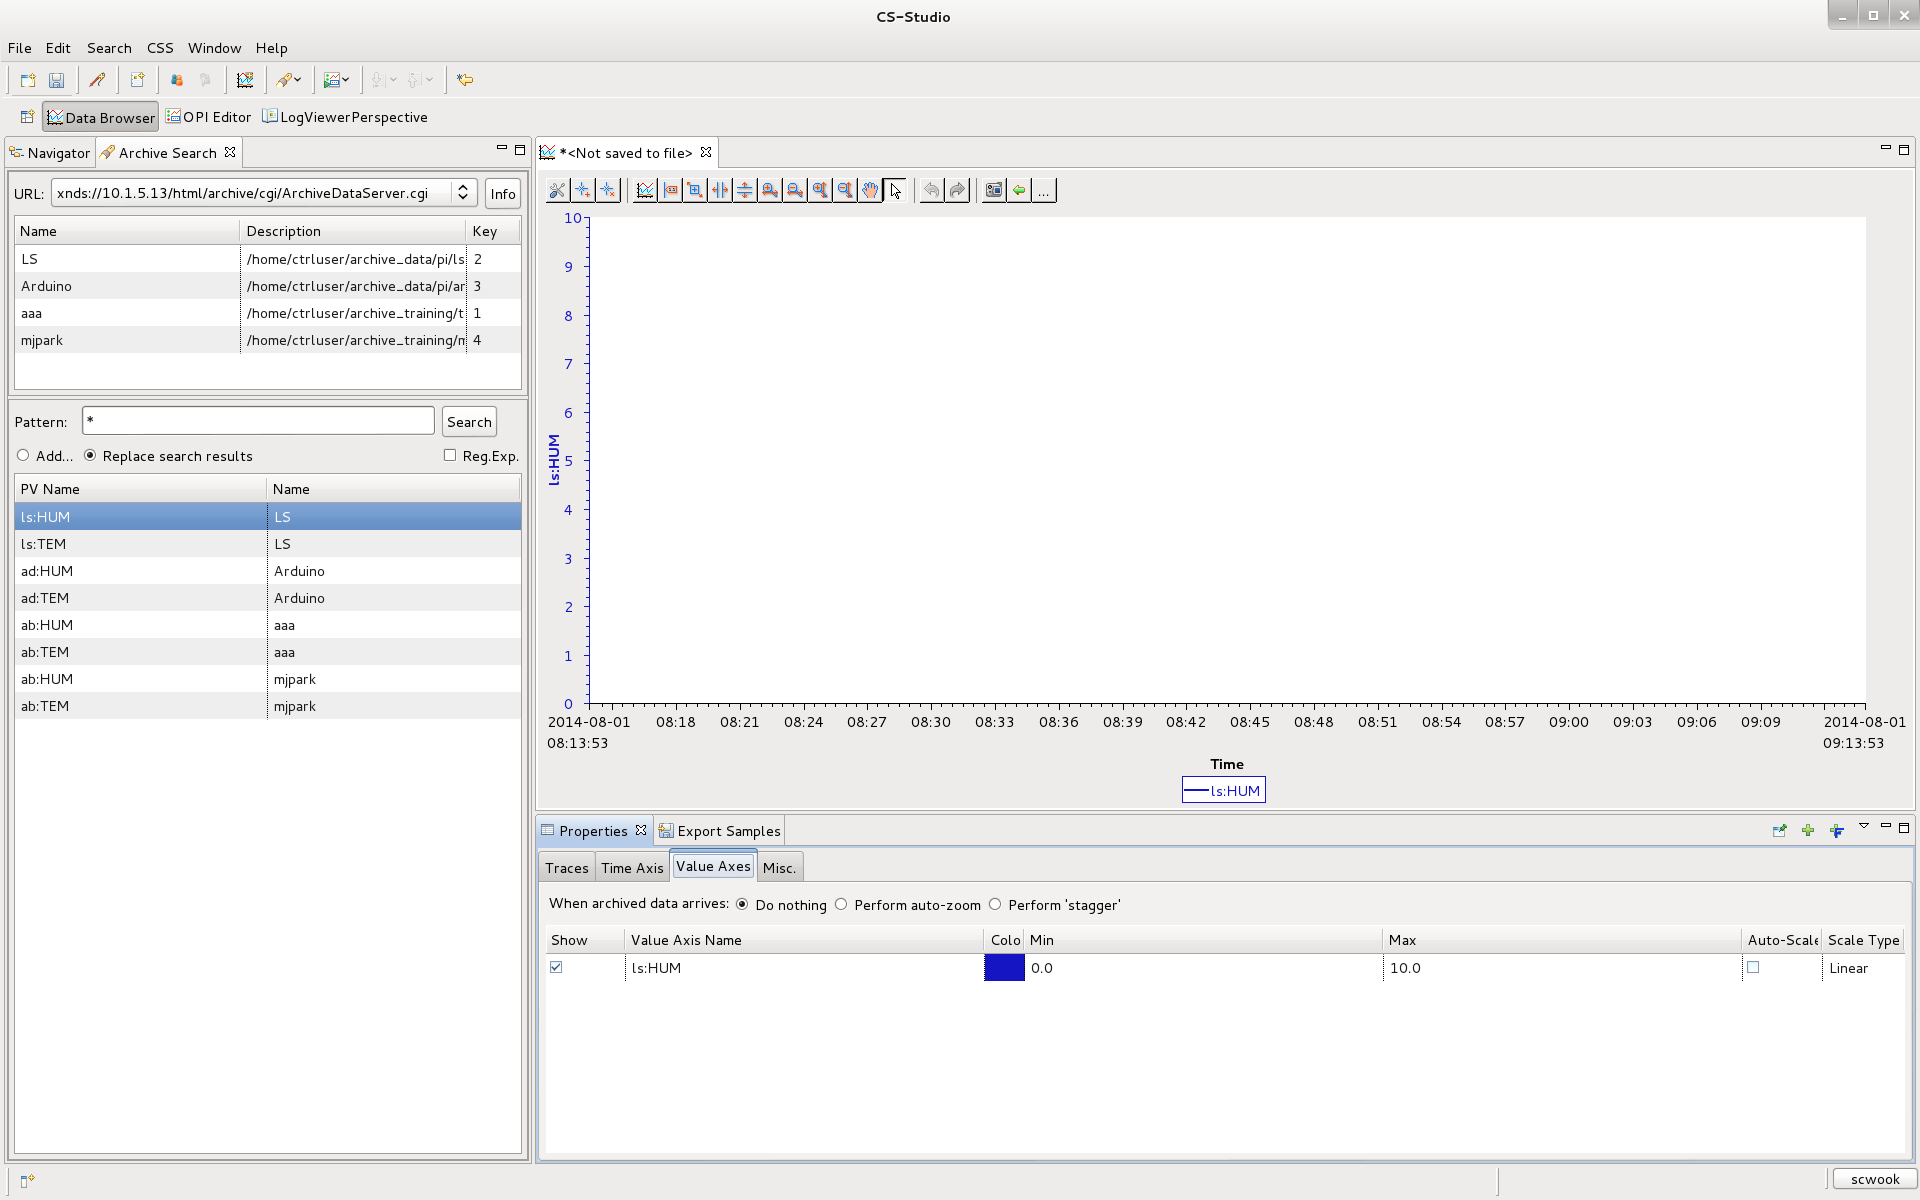
\includegraphics[width=0.96\textwidth]{./images/databrowser.png}
  \caption{
            Data Browser
          }
  \label{fig:css_db}
\end{figure}

%\clearpage
\newpage

\bibliographystyle{unsrtnat}

\bibliography{./refs}

\newpage
\appendix
\newappendix
\label{app:chanarch}
\begin{lstlisting}[style=termstylenumber, caption={chanarch.sh}, label={list:nfsroot-file}]
!/bin/bash
# Shell  : epics_chanarch.sh
# Author : Jeong Han Lee
# email  : jhlee@ibs.re.kr
# Date   : Tuesday, February  4 23:29:02 KST 2014
# version : 0.0.1
#
#    * This script may give a little room to install again-and-again
#      Classic EPICS Channel Archiver located at
#      http://sourceforge.net/projects/epicschanarch/
#
#
#      I hope it would reduce our time to concentrate real works
#      instead of painful modification of unmaintained source codes.
#
#   * Must install the following packages via root or sudo
#     before running this script
#
#     For Debian Wheezy,
#
#      aptitude install libxmlrpc-c++4-dev  libxerces-c-dev  libcurl3-dev
#
#     Of course, EPICS base, and its extension must be installed
#
#
#
#  - 0.0.1  Wednesday, February  5 00:47:14 KST 2014, jhlee
#           * created
#




# cq   : quiet
# c    : continue getting a partially-downloaded file. So it allows us not to re-download an existent file
#
wget_options="wget -c"
# xzf  : quiet
# xzfv : verbose
tar_command="tar xzf"

# aptitude install libxmlrpc-c++4-dev  libxerces-c-dev  libcurl3-dev

make_epicschanarch()
{

    chanarch_dir=$1
    cd ${chanarch_dir}
    echo $PWD
    echo ""
    make_cfg="${chanarch_dir}/make.cfg"
    sed -i~ -e 's/LOCAL=\/usr\/local/LOCAL=\/usr\//g' ${make_cfg}


    # modify Tools in order to compile them correctly
    # Tuesday, February  4 18:42:16 KST 2014, jhlee

    tools_dir=${chanarch_dir}/Tools/
    sed -i~ '$ a\#include <cstdio>\n#include <cstdlib>\n#include <cstdarg>' ${tools_dir}/ToolsConfig.h
    sed -i~ '18istatic int sort_compare(const int &a, const int &b)\n{\n  return b-a;\n}\n\nstatic const char *toString(const int &i)\n{\n  static char txt[10];\n  sprintf(txt, "%d", i);\n return txt;\n }\n' ${tools_dir}/AVLTree.h
    sed -i~ '18,23d'  ${tools_dir}/AVLTreeTest.cpp
    sed -i '5,6d'     ${tools_dir}/AVLTreeTest.cpp

    sed -i -e 's/#include <expat.h>/#include <xmlparse.h>/g' ${tools_dir}/FUX.cpp


    # modify LibIO
    # error: ~@~XLONG_MAX~@~Y was not declared in this scope >> BinValue.cpp
    #./DataFile.h:131:5: error: ~@~XDataHeaderIterator~@~Y does not name a type  >> DataFile.cpp
    #
    libIO_dir=${chanarch_dir}/LibIO/
    sed -i~ '7i#include <climits>\n#include "BinChannelIterator.h"' ${libIO_dir}/BinValue.h


    # modify Storage
    # ../NameHash.cpp:4:23: warning: extra tokens at end of #include directive [enabled by default]

    storage_dir=${chanarch_dir}/Storage/
    sed -i~ -e 's/.h>./.h>/g' ${storage_dir}/NameHash.cpp

    # modify XMLRPCServer
    # Cannot run or decode 'xmlrpc-c-config'
    # ./main_standalone.cpp:81:101: warning: deprecated conversion from string constant to ~@~Xchar*~@~Y [-Wwrite-strings]

    xmlrpcserver_dir=${chanarch_dir}/XMLRPCServer/

    sed -i~ -e 's/1.0/1./g'                       ${xmlrpcserver_dir}/xmlrpc-config-wrapper
    sed -i~ -e 's/"archiver./(char*)"archiver./g' ${xmlrpcserver_dir}/main_standalone.cpp
    sed -i  -e 's/"S:/(char*)"S:/g'               ${xmlrpcserver_dir}/main_standalone.cpp
    sed -i  -e 's/"A:/(char*)"A:/g'               ${xmlrpcserver_dir}/main_standalone.cpp
    sed -i  -e 's/"Get /(char*)"Get /g'           ${xmlrpcserver_dir}/main_standalone.cpp

    # Engine
    # ../hammer.cpp:28:17: error: ~@~Xstderr~@~Y was not declared in this scope
    # ../hammer.cpp:29:58: error: ~@~Xfprintf~@~Y was not declared in this scope
    engine_dir=${chanarch_dir}/Engine/
    sed -i~ -e 's/#include <string>/#include <cstdio>\n#include <cstdlib>\n#include <cstring>\n#include <iostream>/g' ${engine_dir}/hammer.cpp


    cd ${chanarch_dir}
    make
}

chanarch_name="ChannelArchiver"
EXT_SRC=${EPICS_EXTENSIONS}/src


chanarch_filename=epicschanarch.tar.gz
cd ${EXT_SRC}

$wget_options -O ${chanarch_filename} http://epicschanarch.cvs.sourceforge.net/viewvc/epicschanarch/?view=tar
$tar_command ${chanarch_filename} --strip-components=1

#cd ${EXT_SRC}/${chanarch_name}

make_epicschanarch "${EXT_SRC}/${chanarch_name}"
\end{lstlisting}

\newpage
\newappendix
\label{app:AEStart}
\begin{lstlisting}[style=termstylenumber, caption={ArchiveEngineStart.pl}]
#!/usr/bin/perl

$configFile = "engineconfig.xml";

$dirName = ".";

-e $configFile || die "$configFile is not exist. Please use 'makeArchiveEngineConfig.pl'\n";

@psl = `ps aux | grep ArchiveEngine`;

$basePort = 5001;
$machString = "-p $basePort";

foreach $num (0..$#psl)
{
  foreach $idx (0..$#psl)
  {
    if( $psl[$idx] =~ /$machString/ )
    {
      $basePort++;
      $machString = "-p $basePort";
      last;
    }
  }
}

close FH;
\end{lstlisting}

\newpage
\newappendix
\label{app:makeAEConfig}
\begin{lstlisting}[style=termstylenumber, caption={makeArchiveEngineConfig.pl}]

#!/usr/bin/perl

open ( fileHandle, ">engineconfig.dtd" );

print fileHandle <<END_DTD;
<?xml version="1.0" encoding="UTF-8"?>
<!-- DTD for the ArchiveEngine Configuration         -->
<!-- Note that we do not allow empty configurations: -->
<!-- Each config. must contain at least one group,   -->
<!-- and each group must contain at least 1 channel. -->
<!ELEMENT engineconfig ((write_period|get_threshold|
                         file_size|ignored_future|
                         buffer_reserve|
                         max_repeat_count|disconnect)*,
                         group+)>
<!ELEMENT group (name,channel+)>
<!ELEMENT channel (name,period,(scan|monitor),disable?)>
<!ELEMENT write_period (#PCDATA)><!-- int seconds -->
<!ELEMENT get_threshold (#PCDATA)><!-- int seconds -->
<!ELEMENT file_size (#PCDATA)><!-- MB -->
<!ELEMENT ignored_future (#PCDATA)><!-- double hours -->
<!ELEMENT buffer_reserve (#PCDATA)><!-- int times -->
<!ELEMENT max_repeat_count (#PCDATA)><!-- int times -->
<!ELEMENT disconnect EMPTY>
<!ELEMENT name (#PCDATA)>
<!ELEMENT period (#PCDATA)><!-- double seconds -->
<!ELEMENT scan EMPTY>
<!ELEMENT monitor EMPTY>
<!ELEMENT disable EMPTY>
END_DTD

close( fileHandle );

open( fileHandle, ">engineconfig.xml" ) || die "Failed opening.\n";

print fileHandle <<END_XML;
<?xml version="1.0" encoding="UTF-8" standalone="no"?>
<!DOCTYPE engineconfig SYSTEM "engineconfig.dtd">
<engineconfig>
   <write_period>30 sec</write_period>
   <get_threshold>10 sec</get_threshold>
   <file_size>30</file_size>
   <ignored_future>1 hour</ignored_future>
   <buffer_reserve>3</buffer_reserve>
   <max_repeat_count>120</max_repeat_count>
   <group>
      <name>AB</name>
      <channel>
        <name>Pi:bi14</name>
        <period>1 sec</period><scan/>
      </channel>
   </group>
</engineconfig>
END_XML

close( fileHandle );
\end{lstlisting}

\newpage
\newappendix
\label{app:DSConfig}
\begin{lstlisting}[style=termstylenumber, caption={DataServerConfig.py}]
!/usr/bin/python3.2

import os
import sys
import xml.etree.ElementTree as etree

def add_index(root, key, name, path):
    if not os.path.exists(path):
        print("Cannot find the \'index\' file:")
        print(path)
        sys.exit()

    e_archive = root.findall("archive")
    for e in e_archive:
        e_name = e.find("name")
        if e_name.text == name:
           print("%s is already in use, Please select other name" % name)
           sys.exit()

    e_archive = etree.Element("archive")
    etree.SubElement(e_archive, "key").text = key
    etree.SubElement(e_archive, "name").text = name
    etree.SubElement(e_archive, "path").text = path

    root.append(e_archive)

def del_index(root, name):
    e_archive = root.findall("archive")
    exist_name = 0
    for e in e_archive:
        e_name = e.find("name")
        if e_name.text == name:
            root.remove(e)
            print("%s is deleted" % name)
            exist_name = 1

    if not exist_name:
        print("Cannot find the %s" % name)
        sys.exit()

def find_available_key(root):
    e_archive = root.findall("archive")
    available_key = 1
    for num in e_archive:
        for e in e_archive:
            e_key = e.find("key")
            if int(e_key.text) == available_key:
                available_key += 1
                break

    return available_key

def print_usage_error():
    print("\nUSAGE: DataServerConfig [Options] <name>\n")
    print("Options:")
    print("  -a    Add index")
    print("  -d    Delete index")
    print("  -l    Show index list")

def print_archive_list(root):
    e_archive = root.findall("archive")
    for e in e_archive:
        print(e[0].text, e[1].text, e[2].text)

def indent(root, level=0):
    i = "\n" + level*"  "
    if len(root):
        if not root.text or not root.text.strip():
            root.text = i + "  "
        if not root.tail or not root.tail.strip():
            root.tail = i
        for root in root:
            indent(root, level+1)
        if not root.tail or not root.tail.strip():
            root.tail = i
    else:
        if level and (not root.tail or not root.tail.strip()):
            root.tail = i

###########################################################
if len(sys.argv) < 2 or len(sys.argv) > 3:
    print_usage_error()
    sys.exit()

file_name = "serverconfig.xml"
file_path = "/var/www/html/archive/cgi/" + file_name

if not os.path.exists(file_path):
    print("Cannot find the \'%s\' file:" % config_name)
    sys.exit()

root = etree.parse(file_path).getroot()

option = sys.argv[1]
if len(sys.argv) == 2:
    if option == "-l":
        print_archive_list(root)
        sys.exit()
    else:
        print_usage_error()
        sys.exit()
elif len(sys.argv) == 3:
    key_val = str(find_available_key(root))
    name_val = sys.argv[2]
    path_val = os.getcwd() + "/index"
    if option == "-a":
        add_index(root, key_val, name_val, path_val)
    elif option == "-d":
        del_index(root, name_val)
    else:
        print_usage_error()
        sys.exit()
else:
    print_usage_error()
    sys.exit()

indent(root)
etree.ElementTree(root).write(file_path)

with open(file_path, "r") as xml_file:
    data = xml_file.read()

with open(file_path, "w") as config_file:
    config_file.write('<?xml version="1.0" encoding="UTF-8"?>\n<!DOCTYPE serverconfig SYSTEM "serverconfig.dtd">\n')
    config_file.write(data)
\end{lstlisting}

\end{document}
